\documentclass{article}
\usepackage[utf8x]{inputenc}
% \usepackage[english,hebrew]{babel}
% \selectlanguage{English}
\usepackage[top=2cm,bottom=2cm,left=2.5cm,right=2cm]{geometry}
\usepackage{amssymb}
\usepackage{amsmath}
\usepackage{cancel}
\usepackage[dvipsnames]{xcolor}
\usepackage{graphicx} % Add this line to include the graphicx package
\title{Ex2 | Introduction to Networks}
\author{Eran Ston (206704512) \and Oded Vaalany (208230474)}

\date{\today}

\begin{document}

    \maketitle
    \section{Question 1}

    \subsection{subquestion 1}
    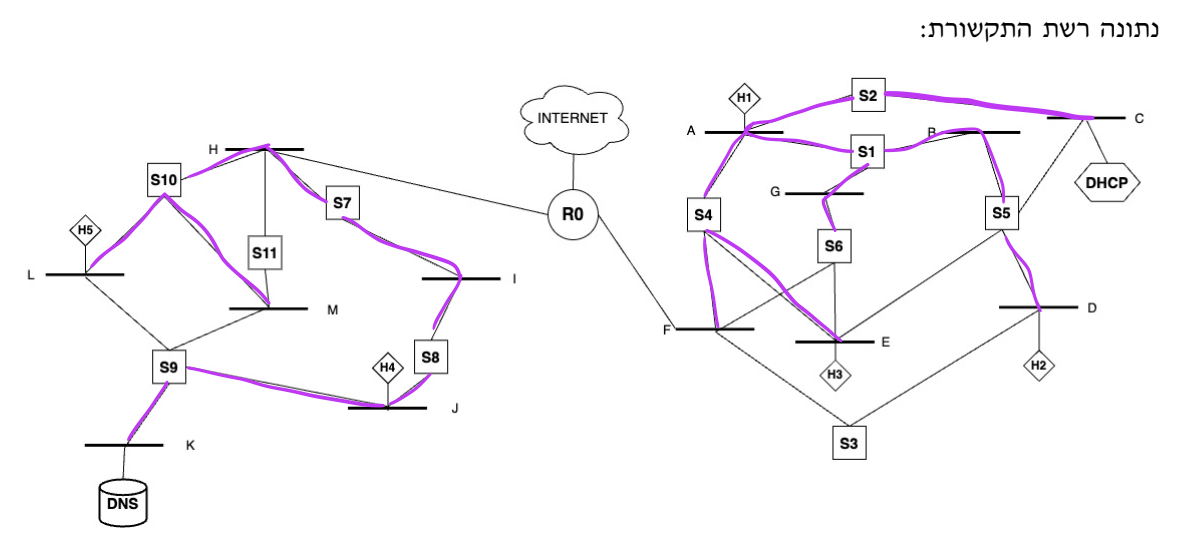
\includegraphics[width=0.9\textwidth]{stp.png}

    There are 2 trees in the network, 
    first tree where s1 is the root and s2,s4,s5 are among the tree but s3,s6 is not in the tree.
    ports of the network are:
    \begin{itemize}
        \item s4 use port 1 
        \item s2 use port 2 
        \item s5 use port 4 
        \item s6 use port 3 
        \item s3 use port 2 
    \end{itemize}

    The second tree where s7 is the root and s8,s10,s11,s9 are among the tree.
    ports of the network are:
    \begin{itemize}
        \item s8 use port 1
        \item s10 use port 1
        \item s11 use port 2
        \item s9 use port 3
    \end{itemize}

    \subsection{subquestion 2}
    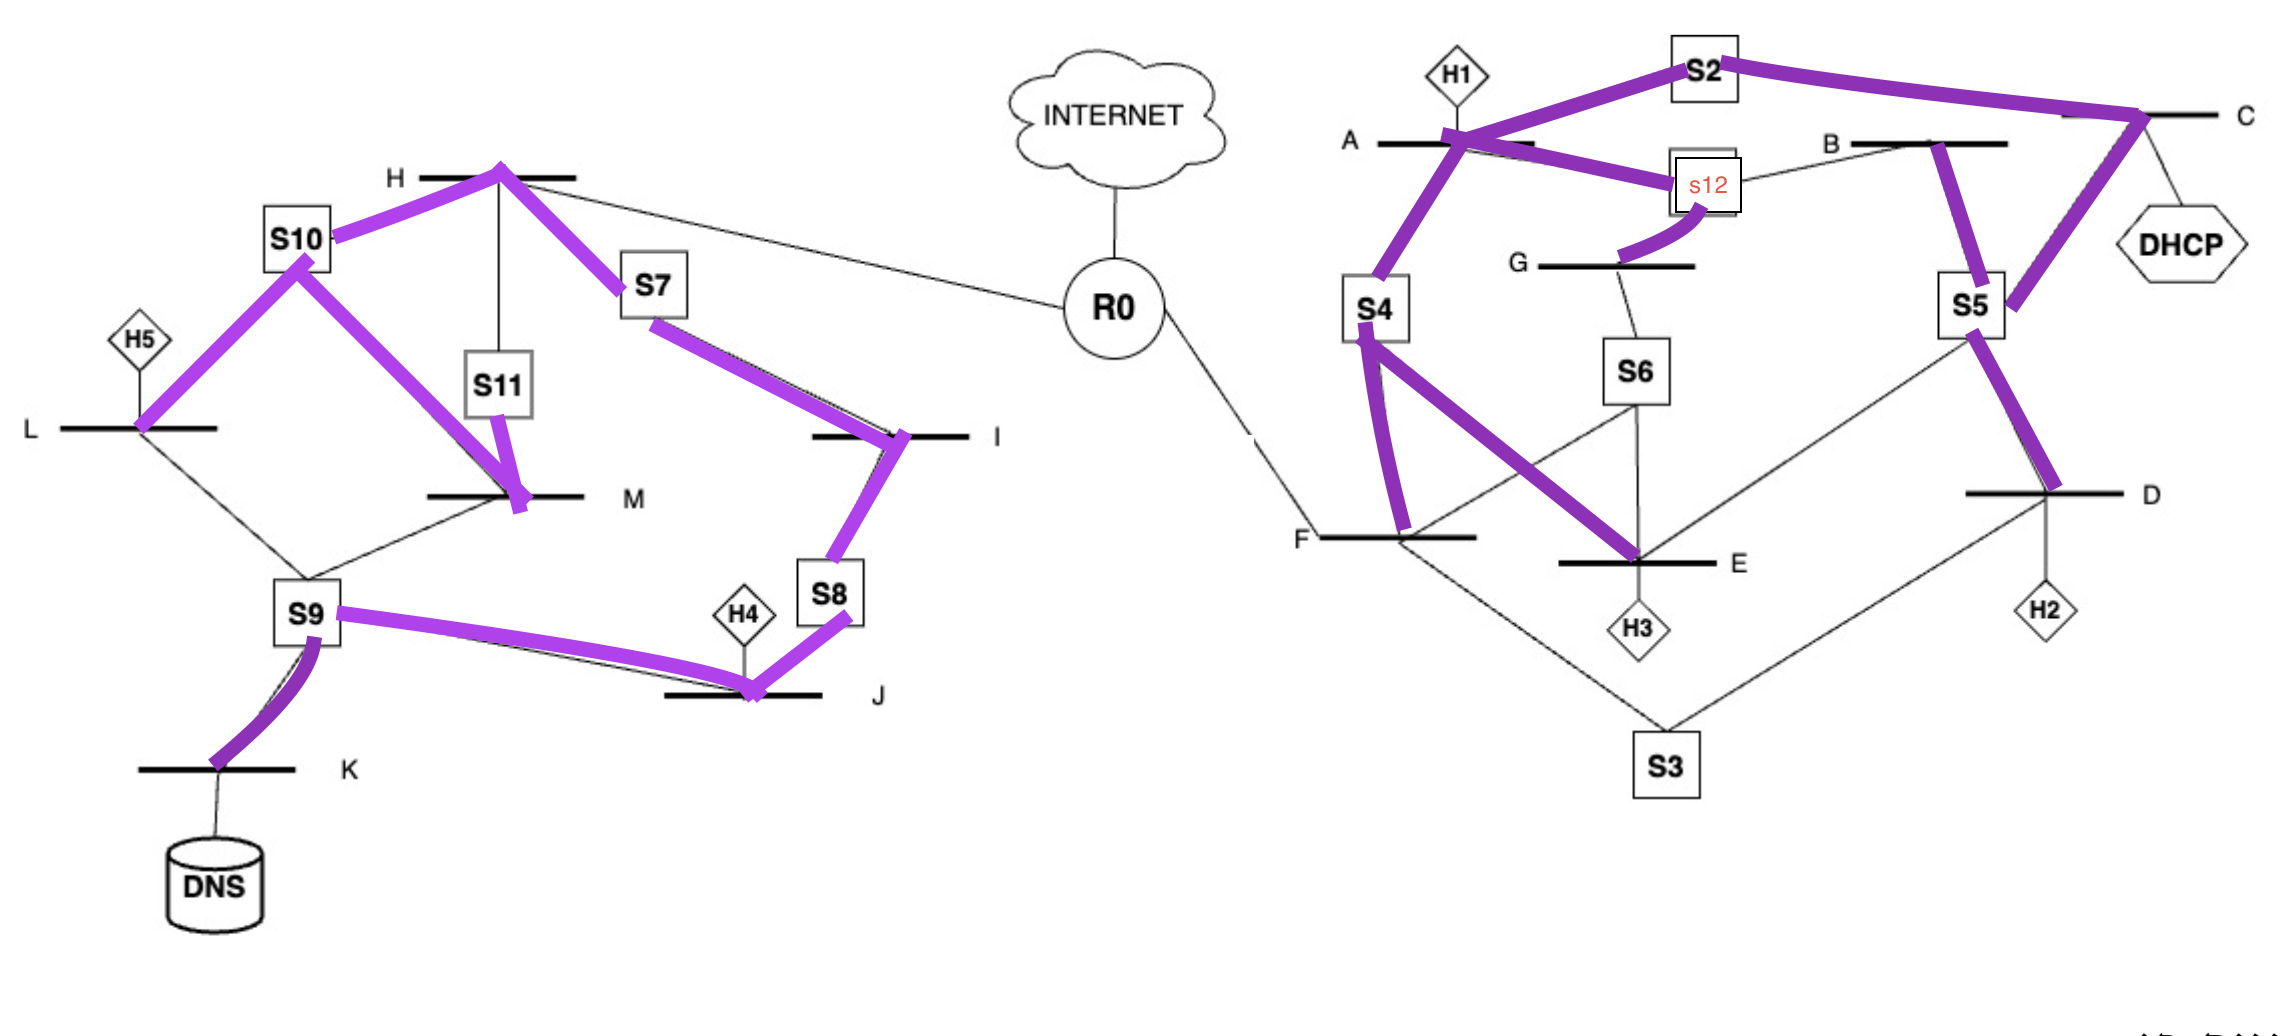
\includegraphics[width=0.9\textwidth]{stp2.png}

    The left tree dosn't change, but the right tree change where s2 is the new root
    s12,s4,s5 are among the tree but s3,s6 is not in the tree.
    ports of the network are:
    \begin{itemize}
        \item s4 use port 1 
        \item s12 use port 3 
        \item s5 use port 2 
        \item s6 use port 2 
        \item s3 use port 2 
    \end{itemize}

    \subsection{subquestion 3}
    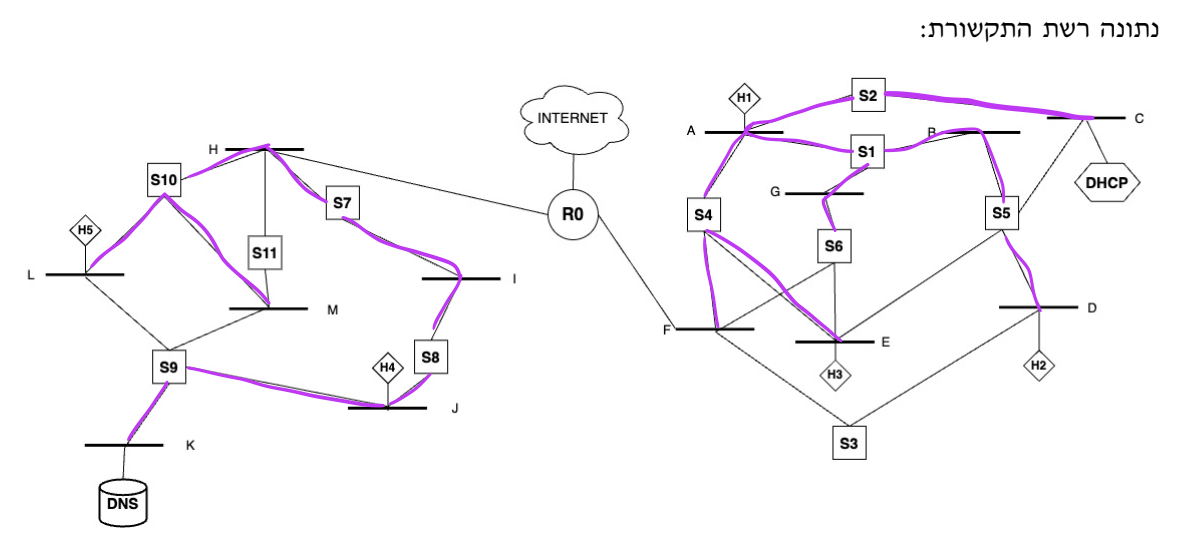
\includegraphics[width=0.9\textwidth]{stp.png}
    \begin{itemize}
        \item H1 $\rightarrow $ H2 - A,B,C,D,E,F,G
        \item H1 $\rightarrow $ H3 - A,B,C,D,E,F,G
        \item H2 $\rightarrow $ H1 - D,B,A
        \item H3 $\rightarrow $ H2 - E,A,F,C,B,D
        \item H4 $\rightarrow $ H5 - J,I,K,H,L,M
    \end{itemize}

    \subsection{subquestion 4}
    \begin{table}[ht]
        \centering
        \begin{tabular}{|c|c|}
            \hline
            \textbf{Host MAC Address} & \textbf{Port} \\
            \hline
            H1 & 3 \\
            \hline
            H2 & 1 \\
            \hline
            H3 & 3 \\
            \hline
        \end{tabular}
    \end{table}

    \section{Question 2}
    \subsection{subquestion 1}
    We have already seen that $T_{out} \geq 2T_{prop}+T_{ack}+T_{pt}$ since the time of processing $T_{pt}$ is neglected and also the time of acknowledgment $T_{ack}$ is neglected, we can say that $T_{out} \geq 2T_{prop}$.
    now we want to calculate $T_{prop }$ since Sam dosen't know the distance between him to the robot therefore we will use 2D as the distance between them. 
    \begin{equation}
        T_{prop} = \frac{2D}{V}
    \end{equation}
    where $V$ is the speed of light and $2D$ is the distance between Sam and the robot.\\



    From mow we will assume that $T_{out} \geq \frac{4D}{V} $
    \subsection{subquestion 2}
    lets donate the distance between Sam and the robot as random variable $Q$.
    as we know the probablity of the robot to go to point 2D is $P(Q=2D) = 0.2$ and the probablity of the robot to go to point D is $P(Q=D) = 0.8$.

    Now we will calculate the $T_{prop}$ where Q = 2D: $T_{prop} = \frac{2D}{V}$ 
    Now we will calculate the $T_{prop}$ where Q = D: $T_{prop} = \frac{D}{V}$ 

    and now we will calculate the expected value of $T_{prop}$:
    \begin{equation}
        E[T_{prop}] = P(Q=2D) \cdot T_{prop} + P(Q=D) \cdot T_{prop} = 0.2 \cdot \frac{2D}{V} + 0.8 \cdot \frac{D}{V} = \frac{1.2D}{V}
    \end{equation}

    \subsection{subquestion 3}
    The probablity of a packet to reach the robot successfully is $P_{success} =  P_{not-error} \cdot P_{not-lost}$ where we know that the probablity to error is p and the probablity to lost is q therefore $P_{success} = (1-p) \cdot (1-q)$

    \subsection{subquestion 4}
    Now we will calculate the goodput of the network:
    \begin{equation}
        \begin{split}
            Goodput &= \frac{T_{packet}}{(\frac{1}{P_{success}}-1)(T_{packet} + T_{out}) + (T_{packet} + 2E[T_{prop}])} \\
        \end{split}
    \end{equation} 

    \subsection{subquestion 5}
    Now we assuming that the probablity for lost is 0 and the probablity for error depends on the distance between Sam and the robot.
    \begin{equation}
        P(Error | Q=2D) = \frac23 \quad P(Error | Q=D) = \frac13
    \end{equation}
    \begin{equation}
        \begin{split}
            P_{success}  &=  (1-P(Error | Q=2D))  \cdot P(Q=2D) + (1-P(Error | Q=D)) \cdot P(Q=D) \\
             &= (1-\frac23)\cdot \frac{1}{5} + (1-\frac13) \cdot \frac{4}{5}\\
             &= \frac{1}{3} \cdot \frac15 + \frac23 \cdot \frac45 \\
             &= \frac{1}{15} + \frac{8}{15}  = \frac9{15} = \frac{3}{5}\\
        \end{split}
    \end{equation}
    
    \begin{equation}
        \begin{split}
            T_{wait \;on\; success} &=  2T_{prop} \\
            T_{wait \;on\; fail} &=  T_{out} \\
            \mathbb{E}[T_{wait}] &= P_{success} \cdot T_{wait \;on\; success} + (1-P_{success}) \cdot T_{wait \;on\; fail} \\
             &= \frac{3}{5} \cdot  2T_{prop} + \frac{2}{5} \cdot T _{out} \\ 
        \end{split}
    \end{equation}

    Now we can calculate the goodput of the network:
    \begin{equation}
        \begin{split}
            Goodput &= \frac{T_{packet}}{T_{wait}+T_{packet}} \\
            &= \frac{T_{packet}}{\frac{6}{5} \cdot  T_{prop} + \frac{2}{5} \cdot T _{out} + T_{packet}} \\
        \end{split}
    \end{equation} 
    \textbf{Note:} $T_{prop}$ is the expected value of the propogation time.

    \section{Question 3}
    \subsection{Part A}
    Let's assume:
    \begin{itemize}
        \item A wants to send 11 packets to B
        \item There is no errors in A's transmission
        \item All the ACK packets B sends to A transmitted successfully and in neglected time.
        \item The processing time in both A and B is neglected.
        \item The time it takes A to send a packet to B is $T_{packet}$
        \item $T_{packet} =T_{prop}$
        \item $_{out}$ from A is the minimal time that can prevent collision
        \item Every fifth packet sent by A is lost
    \end{itemize}
    \subsubsection{subquestion 1}
    \begin{equation}
        T_{out}  = 2T_{prop} + T_{ack} + T_{pt} = 2T_{prop} = 2T_{packet}
    \end{equation}

    \subsubsection{subquestion 2}
    \begin{table}[ht]
        \centering
        \begin{tabular}{|c|c|c|c|c|c|c|c|c|c|c|c|c|c|}
            \hline
            \textbf{Transmission No.} & 1 & 2 & 3 & 4 & 5 & 6 & 7 & 8 & 9 & 10 & 11 & 12 & 13 \\
            \hline
            \textbf{Packet No.} & 1 & 2 & 3 & 4 & 5 & 5 &6 & 7 & 8 & 9 & 9 & 10 & 11  \\
            \hline
        \end{tabular}
    \end{table}
    where the packet number 5 and 9 are lost, and therefore they are sent again.
    
    The time passed from the first packet sent until the last ACK received is:
    \begin{equation}
        T_{transmission}  = \sum^{13}_{i=1} T_{packet} + 2T_{prop} =  3\sum^{13}_{i=1} T_{packet} = 39T_{packet}
    \end{equation}
    
    \subsubsection{subquestion 3}
    Let's assume that the units communicated using Go Back N protocol.
    Since the window size is 3:\\
        \begin{tabular}{|c|c|c|c|c|c|c|c|c|c|c|c|c|c|c|c|c|c|c|c|c|c|c|c|c|c|c|}
            \hline
            \textbf{T} & 1 & 2 & 3 & 4 & \textcolor{red}{5} & 6 & 7 & 8 & 9 & \textcolor{red}{10} & 11 & 12 & 13 & 14 & \textcolor{red}{15} & 16 & 17 & 18 & 19 & \textcolor{red}{20} & 21 & 22 & 23 & 24 & \textcolor{red}{25} & 26\\
            \hline
            \textbf{P} & 1 & 2 & 3 & 4 & 5 & 6 & 7 & 5 & 6 & 7 & 8 & 9 & 7 & 8 & 9 & 10 & 11 & 9 & 10 & 11 & - & - & 11 & - & -  & - \\
            \hline
            \textbf{A} & - & - & - & 1 & 2 & 3 & 4 & - & 6 & 7 & 5 & 6 & - & 8 & 9 & 7 & 8 & - & 10 & 11 & 9 & 10 & - & - & - & 11 \\
            \hline
        \end{tabular}
        \textbf{Note:} '-' is a empty slot , means or we didnt got ack or we didnt send the packet\\\\
        Now we will calculate the time passed from the first packet sent until the last ACK received:
        \begin{equation}
            T_{transmission}  = 25T_{packet}
        \end{equation}
        $T_{packet} = T_{prop}$ from the first massage until the last ACK received. unit A passed 25 transmission epochos. there for the time passed is 25 times the time of a packet.
        
        \subsubsection{subquestion 4}
        
        \begin{tabular}{|c|c|c|c|c|c|c|c|c|c|c|c|c|c|c|c|c|c|c|c|c|c|c|c|c|c|}
            \hline
            \textbf{T} & 1 & 2 & 3 & 4 & {5} & 6 & 7 & 8 & 9 & {10} & 11 & 12 & 13 & 14 & {15} & 16 & 17 & 18\\
            \hline
            \textbf{P} & 1 & 2 & 3 & 4 & \textcolor{red}5 & 6 & 7 & 5 & - & - & 8 & \textcolor{red} 9 & 10 & 11 & 9 & - & - & - \\
            \hline
            \textbf{A} & - & - & - & 1 & 2 & 3 & 4 & - & 6 & 7 & 5 & - & - & 8 & - & 10 & 11 & 9      \\
            \hline
        \end{tabular}
        \begin{equation}
            T_{transmission}  = 17T_{packet}
        \end{equation}
        $T_{packet} = T_{prop}$ from the first massage until the last ACK received. unit A passed 17 transmission epochos. there for the time passed is 17 times the time of a packet.

        \subsection{Part B}
        In this part we will assume:
        \begin{itemize}
            \item A wants to send 8 packets to B
            \item Window size is 6
            \item $T_{out}$ of A equal to the time A needs to send 5 packets
            \item All the ACK packets B sends to A transmitted successfully.
            \item Let's assume that in time of sending packets sum of 5 packest are lost.
        \end{itemize}
        \subsubsection{subquestion 1}
        \begin{tabular}{|c|c|c|c|c|c|c|c|c|c|c|c|c|c|c|c|c|c|c|c|c|c|c|c|c|c|}
            \hline
            \textbf{T} & 1 & 2 & 3 & 4 & {5} & 6 & 7 & 8 & 9 & {10} & 11 & 12 & 13 & 14 & {15} & 16 & 17 & 18 & 19 & {20} & 21 & 22 & 23 & 24 & {25}  \\
            \hline
            \textbf{P} & 1 & \textcolor{red}2 & \textcolor{red}3 & \textcolor{red}4 & \textcolor{red}5 & \textcolor{red}6 & 7 & 2 & 3 & 4 & 5 & 6 & 7 & 8\\
            \hline
            \textbf{A} & - & - & - & - & - & - & 1 & - & - & - & - & - & 2 & 3 & 4 & 5 & 6 & 7 & 8 \\
            \hline
        \end{tabular}
        First we send 6 packet if the last 5 packets in the window are lost we send the 5 packets again and a new packet in the end.\\ 
        after that there is no packets that are lost so we send the rest one after the other, this gives us that the number of packets that\\
        that are transmited again is 5.\\
        
        \subsubsection{subquestion 2}
        \begin{tabular}{|c|c|c|c|c|c|c|c|c|c|c|c|c|c|c|c|c|c|c|c|c|c|c|c|c|c|}
            \hline
            \textbf{T} & 1 & 2 & 3 & 4 & {5} & 6 & 7 & 8 & 9 & {10} & 11 & 12 & 13 & 14 & {15} & 16 & 17 & 18 & 19 & {20} & 21 & 22 & 23 & 24 & {25}  \\
            \hline
            \textbf{P} & \textcolor{red}1 & 2 & 3 & 4 & 5 & 6 & \textcolor{red}1 & 2 & 3 & 4 & 5 & 6 & \textcolor{red}1 & 2 & 3 & 4 & 5 & 6 & \textcolor{red}1 & 2 & 3 & 4 & 5 & 6 & \textcolor{red}1\\
            \hline
            \textbf{A} & - & - & - & - & - & - & - & 2 & 3 & 4 & 5 & 6 & - & 2 & 3 & 4 & 5 & 6 & - & 2 & 3 & 4 & 5 & 6 & -  \\
            \hline
        \end{tabular}

        \begin{tabular}{|c|c|c|c|c|c|c|c|c|c|c|c|c|c|c|c|c|c|c|c|}
            \hline
             26 & 27 & 28 & 29 & 30 & 31 & 32 & 33 & 34 & 35 & 36 & 37 & 38 & 39 & 40 & 41 & 42 & 43 & 44 \\
            \hline
            2 & 3 & 4 & 5 & 6 & 1 & 2 & 3 & 4 & 5 & 6 & 7 & 8 & - & - & - & - & - & -\\
            \hline
            2 & 3 & 4 & 5 & 6 & - & 2 & 3 & 4 & 5 & 6 & 1 & 2 & 3 & 4 & 5 & 6 & 7 & 8 \\
            \hline
        \end{tabular}
        In this example we send packets number 1,2,3,4,5,6 again and again 5 times until we get the ACK from the last packet. so we sends 30 packets again.\\

        \textbf{Note:} from now on we will use selectiv repeat protocol.\\
        \subsubsection{subquestion 3}
        \begin{tabular}{|c|c|c|c|c|c|c|c|c|c|c|c|c|c|c|c|c|c|c|c|c|c|c|c|c|c|}
            \hline
            \textbf{T} & 1 & 2 & 3 & 4 & {5} & 6 & 7 & 8 & 9 & {10} & 11 & 12 & 13 & 14 & {15} & 16 & 17 & 18 & 19 & {20}   \\
            \hline
            \textbf{P} & 1 & 2 & 3 & \textcolor{red}4 & \textcolor{red}5 & \textcolor{red}6  & \textcolor{red}7 & \textcolor{red}8 & - & 4 & 5 & 6 & 7 & 8 & -  & - & - & - & - & -\\
            \hline
            \textbf{A} & - & - & - & - & - & - & 1 & 2 & 3 & - & - & - & - & - & - & 4 & 5 & 6 & 7 & 8\\
            \hline
        \end{tabular}\\
        In this example we send packets number 4,5,6,7,8,6 again just one time , so we send 5 packets again. (the protocol sends again only packets that fail)\\
        
        \subsubsection{subquestion 4}
        Since selectiv repeat protocol transmit packet again only if its ack is not received we can say that the the max number of retransmited packet is as same as the number that lost and therefore only 5 packets were retransmited
        \subsubsection{subquestion 5}
        The protocl desont "care" if the packet is lost or the ack is lost , it act the same for both , so the number of packets that the protocol will send again is then number of failed\\
        packets + acks , so total 5 packets will be retransmited.
        \end{document}